\section{任务一}
本任务分成两个部分，先是创建10个进程/线程，其中5个占用70\%的CPU，5个占用30\%的CPU。
另外一个任务是创建一个实时进程，观察是否会影响到其他进程的运行。

\subsection{子任务一}

我们将创建一个CPU集合，并且只包含CPU的0号核心，以便于之后进程绑定核心。

\begin{lstlisting}[language=C]
    cpu_set_t cpuset;
    CPU_ZERO(&cpuset);
    CPU_SET(0, &cpuset);
\end{lstlisting}

创建进程的方式使用的是C语言标准库的fork函数，创建之后
使用\texttt{sched\_setaffinity}函数将进程绑定到CPU的0号核心上。
接下来是通过进程id的不同，选择前半部分设置高优先级，后半部分设置低优先级。
优先级的设置方式是nice value。
我一开始设置的是-10和10，但是发现这样高优先级的占据了95\%的CPU，低优先级的几乎没有CPU使用率。
然后我逐渐微调，发现-3和1的组合较为合适。
设置完优先级之后，我们需要创建一个CPU密集型的任务让进程不断的执行。
在这里我写了一个简单的死循环加法，为了保证不溢出，每次的计算结果都会取模。

为了保证创建子进程的父进程不提前退出，我们需要在创建
完进程之后通过waitpid函数等待子进程的结束。

如此就完成了第一部分的任务。通过top指令可以得到如图~\ref{fig:normalRun}和~\ref{fig:normalTop}的效果截图
\begin{figure}[!h]
    \centering
    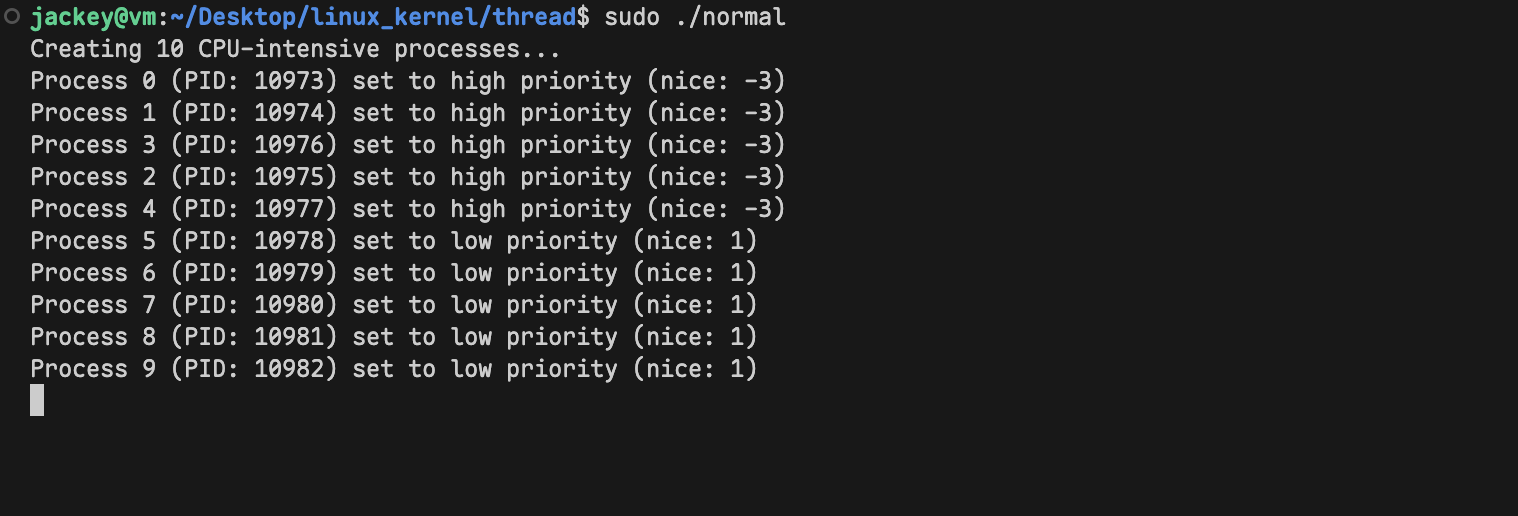
\includegraphics[width=0.5\textwidth]{../fig/normalRun.png}
    \caption{程序运行截图}
    \label{fig:normalRun}
\end{figure}

\begin{figure}[!h]
    \centering
    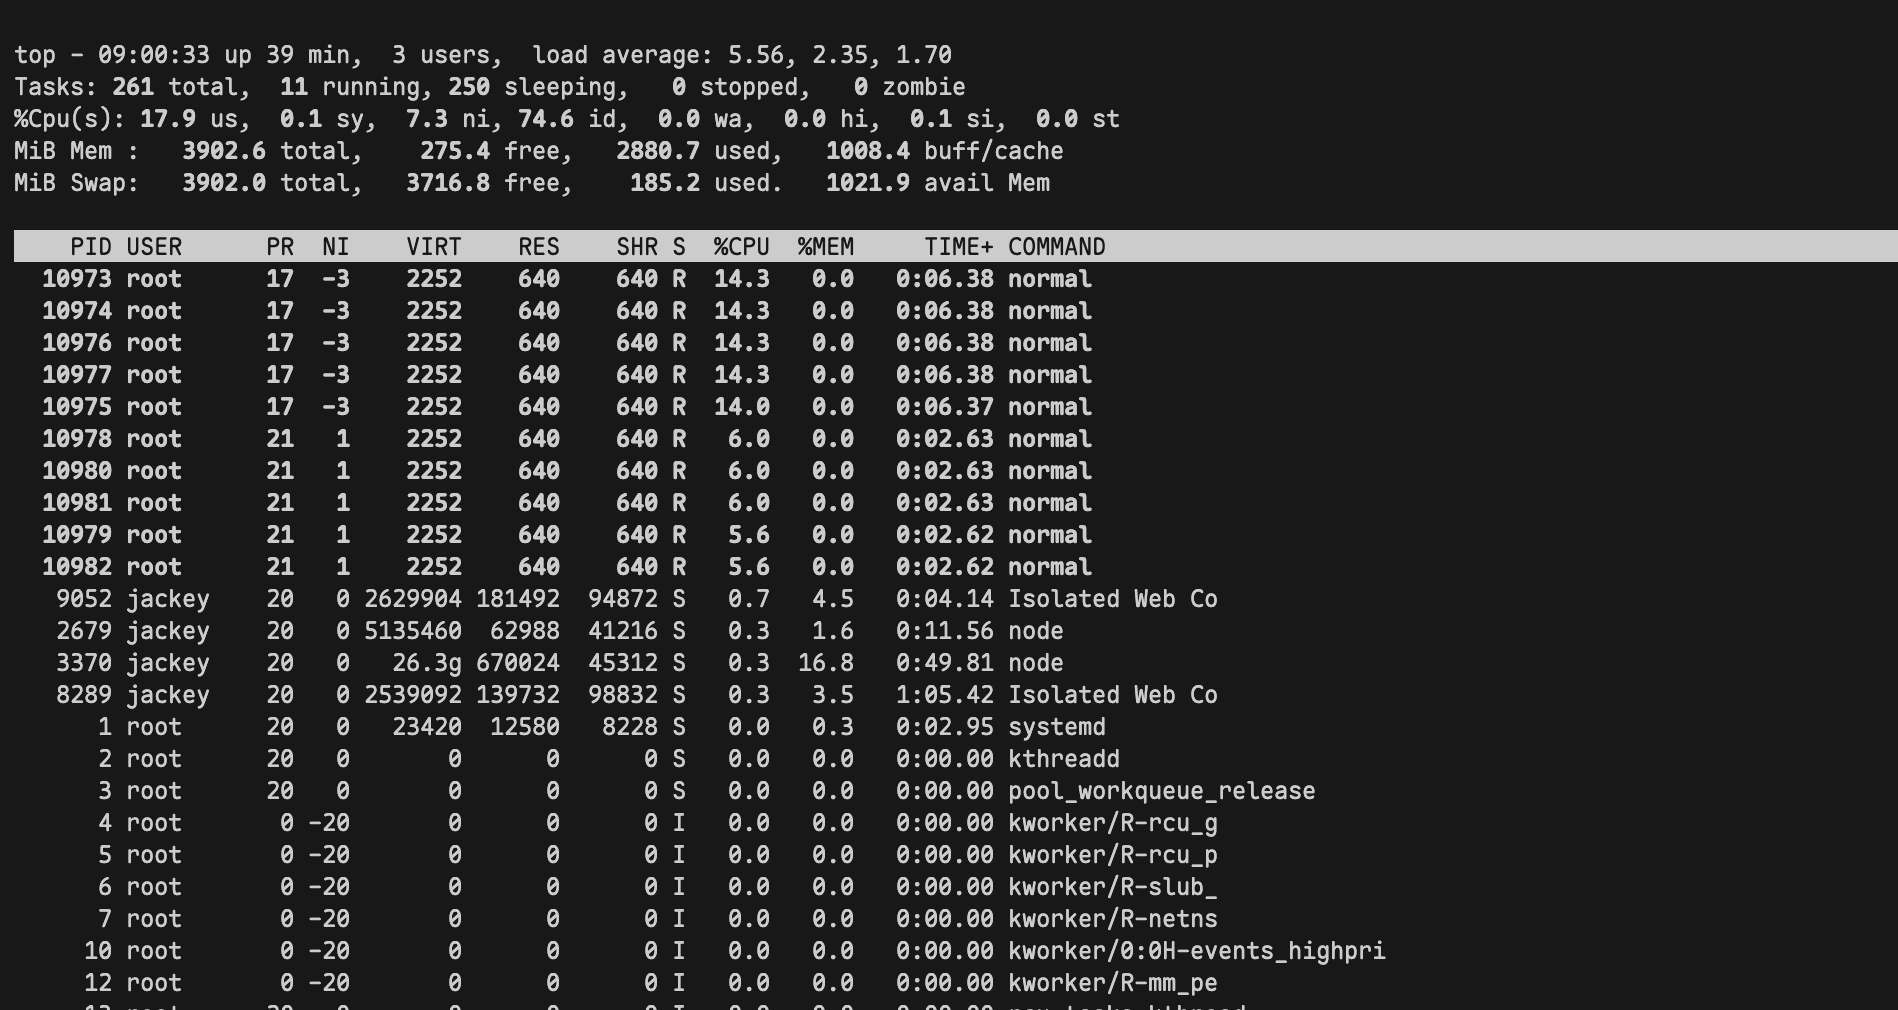
\includegraphics[width=0.6\textwidth]{../fig/normalTop.png}
    \caption{top指令截图}
    \label{fig:normalTop}
\end{figure}

\subsection{子任务二}

本部分创建CPU Set的方式和上述一致。本部分唯一的不同之处在于创建的
进程是实时进程，使用\texttt{sched\_setscheduler}来设置优先级。
考虑到实时进程的优先级是0-99，为了让抢占的效果更好，我们直接将
优先级设置成最高的99。对应的代码是
\begin{lstlisting}[language=C]
    struct sched_param param;
    param.sched_priority = 99; 
    if (sched_setscheduler(0, SCHED_RR, &param) != 0) {
        perror("sched_setscheduler failed");
        exit(1);
    }
\end{lstlisting}

创建完进程之后，我们同样使用死循环加法来占用CPU资源。
我们笼统的使用\texttt{wait(NULL)}来等待实时进程的结束。

如此，我们得到了如图~\ref{fig:realRun}和~\ref{fig:realTop}的效果截图，可以看到
实时进程基本占用了所有的CPU资源。

\begin{figure}[!h]
    \centering
    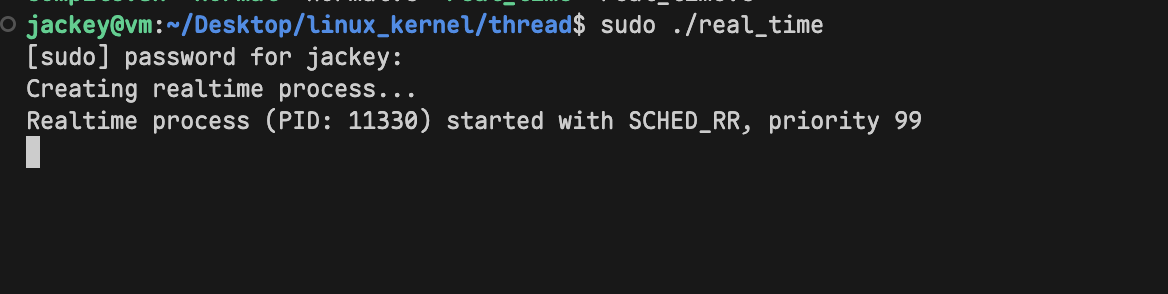
\includegraphics[width=0.5\textwidth]{../fig/realRun.png}
    \caption{程序运行截图}
    \label{fig:realRun}
\end{figure}

\begin{figure}[!h]
    \centering
    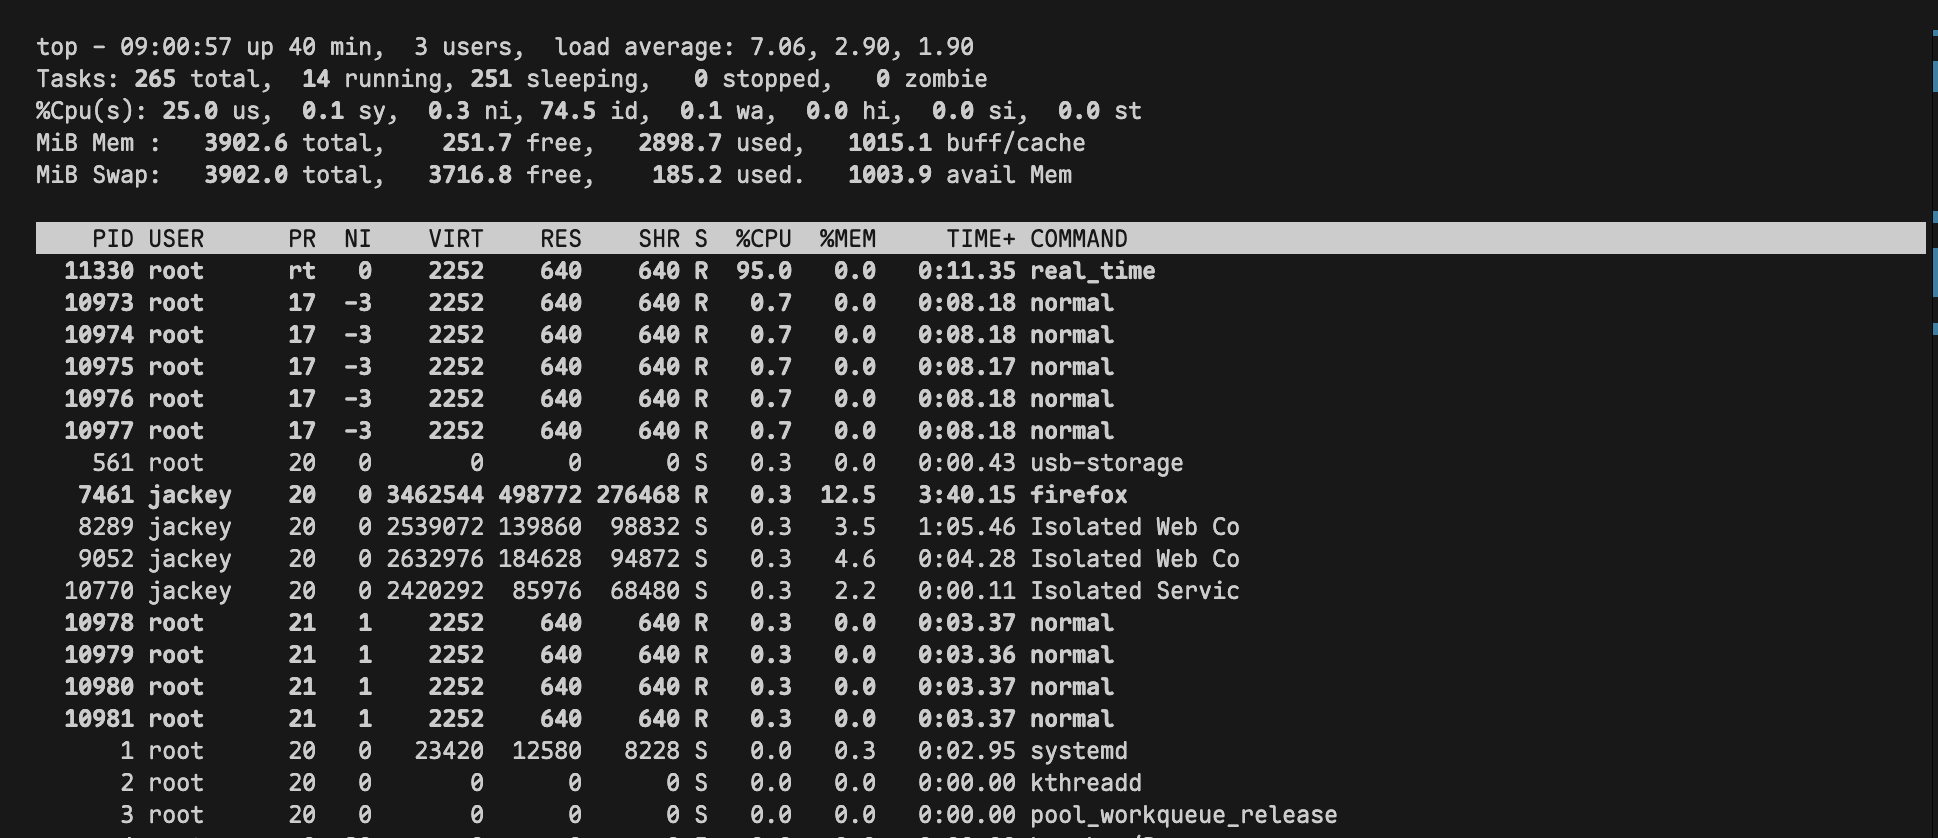
\includegraphics[width=0.6\textwidth]{../fig/realTop.png}
    \caption{top指令截图}
    \label{fig:realTop}
\end{figure}

\subsection{编译}
在上传的代码文件中包含了运行脚本\texttt{compile.sh}，该文件就是简单的gcc编译的过程。
运行可执行文件时需要注意root权限。

\subsection{MISC}
我一开始用Rust艰难的写了一版，但忘记commit了。然后我在
跑第二部份的代码的时候遇到了虚拟机内存不够的问题。我调大了
虚拟机的内存，结果导致了虚拟机无法启动。最后我只能装了个Ubuntu，从头来过。

\section{任务二}
本部分选择的是linux内核6.6.87版本。因为没有在下载kernel代码的时候
init git，导致我写完之后没法生存patch，所以我在我每处修改的地方
都加了\texttt{I Modify Here}的注释，可以方便的定位。

本部分的要求可以拆分成两点，记录进程调度的次数，并且将其写到proc文件系统中的
ctx文件之中。

我们先看第一个任务，我们需要在进程中用一个变量记录当前被调度的次数，
而内核中用来表示线程的数据结构是sched.h中的\texttt{task\_struct}。
我添加了一个unsigned long类型的变量\texttt{sched\_count}。

那么在哪里初始化这个变量呢？我们知道进程都是fork出来的，所以就应该找到
fork的源码，其在kernel/fork.c中的\texttt{copy\_process}函数中。
从返回值可以看出p就是新创建的子进程，那么只要添加\texttt{p->sched\_count = 0}即可。我
的代码写在第2594行。

接下来我们需要在调度的时候动态的修改这个值。
调度的时候调用的是core.c中的\texttt{context\_switch}函数。
原来的进程是\texttt{prev}，新的进程是\texttt{next}，
我们只需要在函数返回前添加\texttt{next->sched\_count += 1}即可。
我的代码写在第5381行。

最后我们需要修改文件系统，创建一个proc文件系统的文件ctx，并在读取
该文件的时候打印出当前进程的调度次数。
我们先观察base.c中的\texttt{pid_entry}结构，这是proc文件系统
中每个文件注册的地方，因为ctx只是一个普通的文件，所以用REG宏创建即可。
因为要求ctx是只读文件，所以权限选的是0444，对应的是S_IRUGO。
我们需要自定义ctx的\texttt{file_operations}结构体。其中只要指定我们需要的
文件打开，读取和lseek的函数即可。但我们其实只需要
自定义读就行，文件打开用\texttt{single\_open}，lseek用\texttt{generic\_file\_llseek}。

最后最关键的是读取函数，我们的目标是根据一个file结构体，通过inode获得进程信息，将进程的被调用次数的变量
复制到用户态的buffer之中。函数的原型可以参考base.c中其他读取函数的原型。
我写的代码如下，代码中包含了如上分析的注释。
\begin{lstlisting}[language=C]
    static ssize_t proc_ctx_read(struct file *file, char __user *buf, size_t len, loff_t *ppos)
    {   
        // get task_struct from file
        struct task_struct *task = get_proc_task(file_inode(file));
        char tmp[32];
        size_t tmp_len;
    
        if (!task)
            return -ESRCH; 

        // copy to temp buffer
        tmp_len = snprintf(tmp, sizeof(tmp), "%lu\n", task->sched_count);

        // release task_struct
        put_task_struct(task);
    
        // copy to user buffer
        return simple_read_from_buffer(buf, len, ppos, tmp, tmp_len);
    }
\end{lstlisting}


最后进行实验验证，使用的是实验要求中提供的死循环C代码，在\texttt{test.c}中。重新编译内核并且按教程中所示的方法安装后，可以得到图~\ref{fig:kernel}所示的结果。
从图中可以看出，在用户没输入字符的时候，文件被调度了一次。每输入一个字符的时候，就又被调度了一次，符合预期。

\begin{figure}[!h]
    \centering
    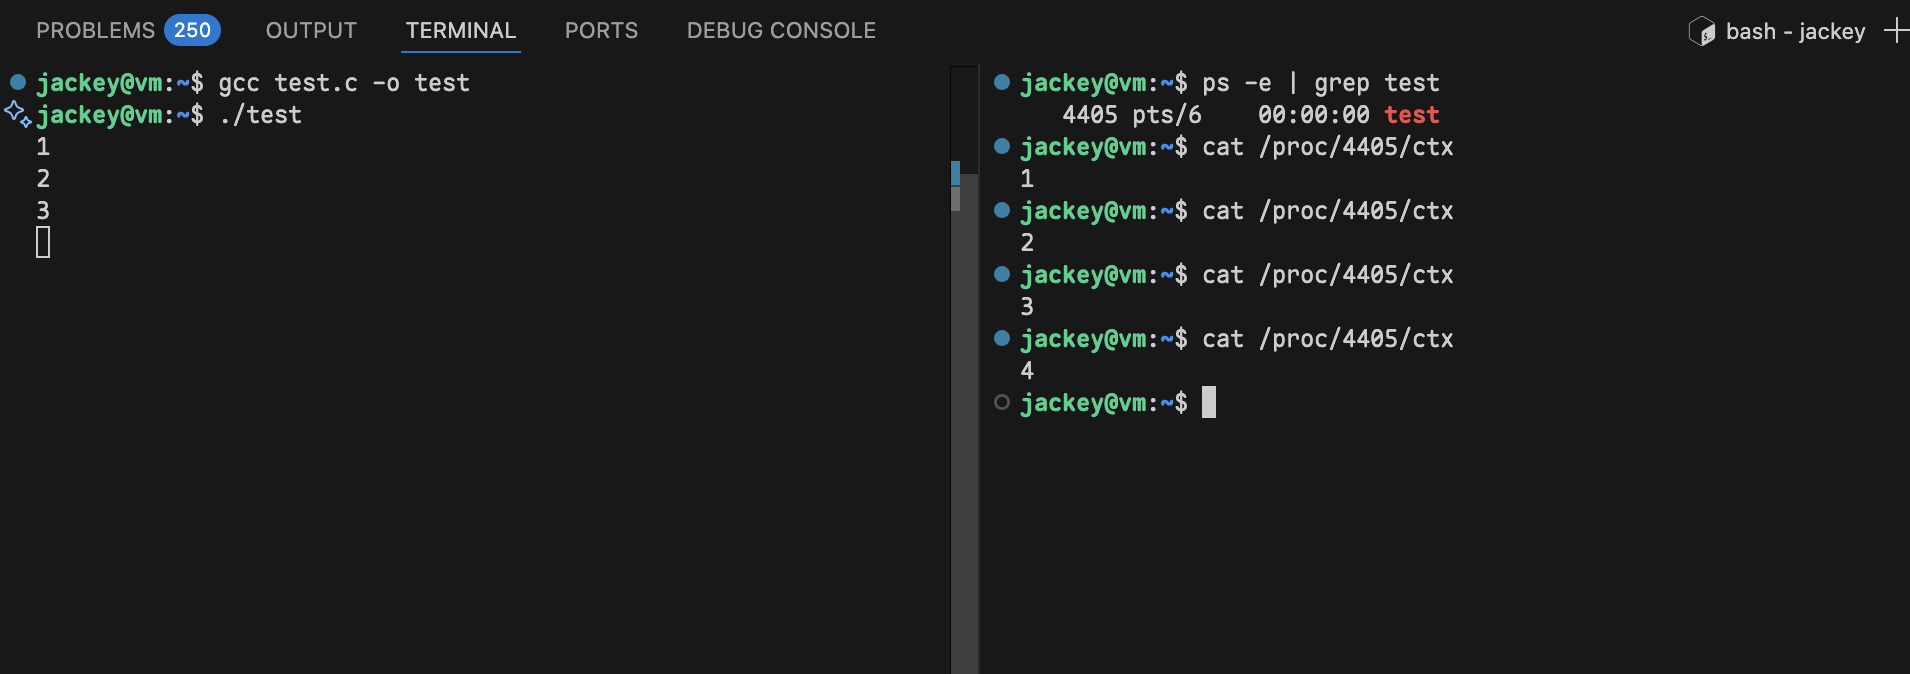
\includegraphics[width=0.8\textwidth]{../fig/kernel.png}
    \caption{内核调度次数}
    \label{fig:kernel}
\end{figure}

编译\texttt{test.c}的方式就是在命令行执行\texttt{gcc test.c -o test}。

\section{MISC}
本部分的代码仍然托管在 \href{https://github.com/JackeyHua-SJTU/linux-kernel}{Github}上。